\pagebreak
\subsection{Electrical Design}

\begin{centering}
The electronics design can be seen in Figure \ref{fig:electronics-block-diagram}. There will be three distinct areas, the Electronics box, the AAC system and the CAC system. All connections to the outside of the box are located in the electronics box. These are the voltage regulators for the external power source and the Ethernet shield with an SD data storage which will connect to the Telemetry, Tracking, and Command (TT\&C). Additionally a pressure sensor, a heater and a temperature sensor will be placed in this area. The CAC system area will only contain one heater to maintain its temperature and one electronic valve to be closed before landing. In the AAC system area there will be the air pump, valves, airflow sensor, pressure sensor, temperature and humidity sensor and a heater.
\end{centering}
\bigskip

\begin{figure}[H]
    \begin{align*}
        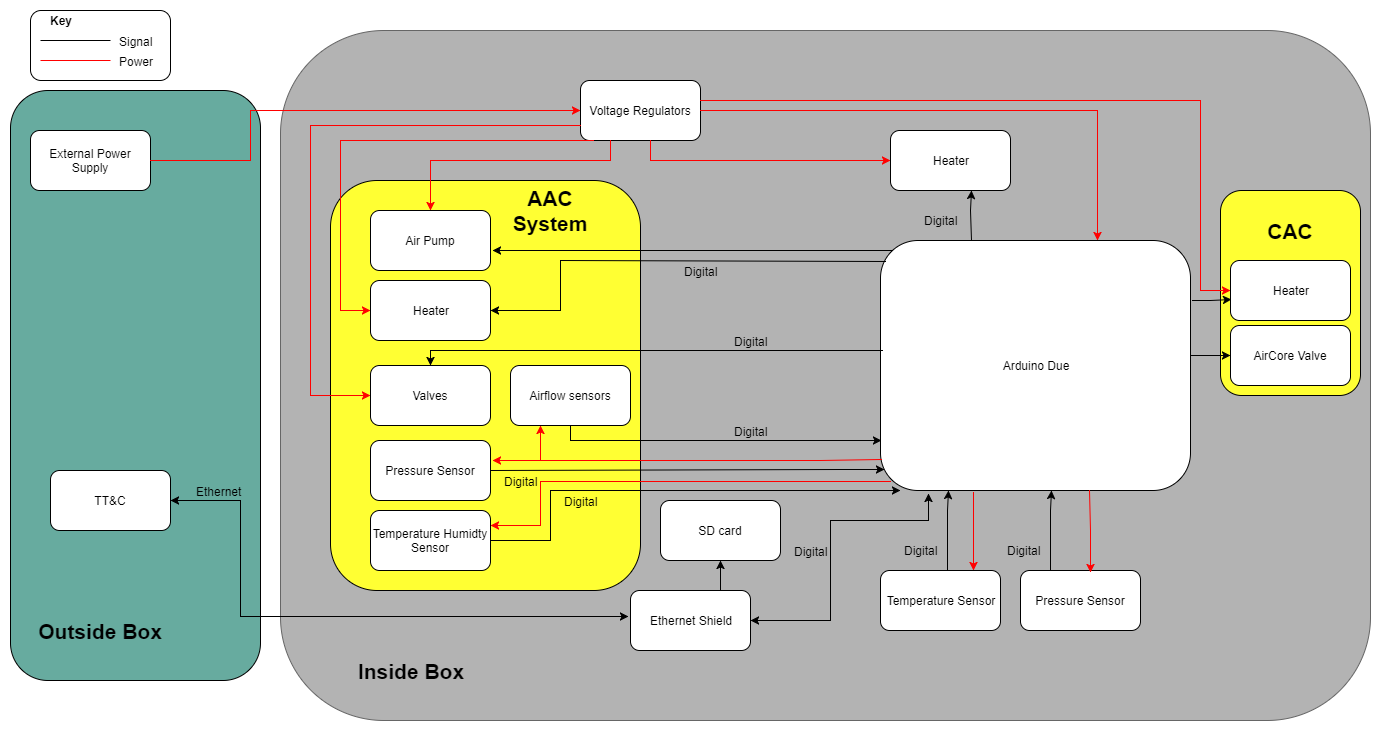
\includegraphics[width=16cm]{4-experiment-design/img/electrical-block-diagram.png}
    \end{align*}
    \caption{Block Diagram for all Electronic Components and Connections}\label{fig:electronics-block-diagram}
\end{figure}

\begin{centering}
Voltage regulators will be used to step down the voltage from the 28.8V provided by the gondola down to: 
\end{centering}

\begin{centering}
\begin{itemize}
  \item $28.8V \Longrightarrow 12V$ for the Arduino.  
  \item $28.8V \Longrightarrow 24V$ for the pump and valves.
  \end{itemize}

\end{centering}
\bigskip

\begin{centering}
The heaters will not require the voltage to be stepped down and so will be powered directly from the gondola battery.
\end{centering}
\bigskip


\raggedbottom